\chapter{Trajectory Following}
\label{chapter:following}

Given a reference state trajectory $\hat{x}_k=\left\langle x_0, x_1, \ldots, x_k \right\rangle$ obtained for a fixed time step $\Delta t$ and a current state of the vehicle estimated from sensor readings using a localization and odometry algorithm, our task is to define a function which will select the next action $u\in U$ such that the car will move in a way in which it will follow the reference trajectory ``as closely as possible''. We will also consider avoiding any obstacles which were not known during the planning phase and which might have been hit if we had followed the trajectory blindly.

In this chapter, we will first formally define what we mean by following the trajectory ``as close as possible''. We will then describe algorithms which we will later implement and try on the experimental vehicle.

\section{Reference State and Sub-trajectory}

First, we must consider the timing of the next control input we will use. The last known vehicle state estimation $x_t\in X$ at time $t$ could be used directly to calculate the error from the reference trajectory. The decision process will take some time $t_d>0$, during which the vehicle will continue to move subject to the last control input $u\in U$. As a consequence of this delay, at the time $t+t_d$ it might not be appropriate to use the action selected by the trajectory tracking algorithm anymore.

To achieve better accuracy, we can estimate the decision delay $t_d$ by averaging the reaction times of the selected algorithm gathered during experiments. We can use our system simulator to estimate the state of the vehicle at the time $t+t_d$. when the action should be applied. We will therefore use the predicted state $x_{pred}=f_{t_d}(x_t,u)$ to find a corresponding state on the reference trajectory to calculate an error.

We must determine what part of the trajectory we have already followed and what is still remaining to be followed.  For the predicted state of the vehicle $x_{pred}$, we will select its reference state along the reference trajectory $\hat{x}_k$ as the state, which is closest to the current location. In the ideal case, this would be one of the states along the reference trajectory or a state between two adjacent states. In practice, the vehicle will deviate from the reference trajectory due to sensing and steering imperfections, but we assume that it is still near the reference trajectory. When the vehicle deviates too much, we assume that the trajectory will be re-planned with respect to the current state of the vehicle. The following function describes how we find the reference state $x_{ref}$:

\begin{equation}
\begin{aligned}
x_{ref}(x_{pred}, \hat{x}_k)&=\argmin_{x_i \in \hat{x}_k} \norm{\kappa_{x,y}(x_{pred})-\kappa_{x,y}(x_i)},
\end{aligned}
\end{equation}
	
where $\kappa_{x,y}: X\rightarrow \mathbb{R}^2$ is the function we defined in Section~\ref{sec:configuration_and_state_space} which returns the position vector in the given state.

We will consider the reference state to be the point which splits the trajectory into the already traveled part and the rest. If $i$ is the index of the reference state in $\hat{x}_k$, then the reference sub-trajectory which should still be followed is $\hat{x}_{ref}=\left\langle x_i, x_{i+1}, \ldots, x_k \right\rangle$.

\section{Trajectory Tracking Error}

To evaluate which control input to select and to evaluate the choice of this input, we must define an error function $e: X\times X\rightarrow \left[0, 1\right]$ which tells us how far apart the two states are from each other. This function will allow us to compare vehicle states between each other and determine which one of them is better. We will also define a second error $\hat{e}_{\Delta t}: X^*\times X^*\rightarrow \left[0, 1\right]$ function to calculate an error between two sequences of states.

\subsection{Single State Error}

We will calculate the error between two states by combining three components: position error, heading error, and velocity error.

\subsubsection{Position Error}

The position error is simply the distance from the desired location:

\begin{equation}
	\label{eq:position_error}
	e_p(x, x_{ref})=\dfrac{\norm{\kappa_{x,y}(x)-\kappa_{x,y}(x_{ref})}}{w},
\end{equation}

where $w\in \mathbb{R}$ is a normalization constant which represents the maximum possible position error for the given track.

\subsubsection{Heading Error}

The heading error is the misalignment of the current heading angle and the heading angle in the reference state:

\begin{equation}
\label{eq:heading_error}
\begin{aligned}
	\Delta \theta(x, x_{ref}) &= |\kappa_\theta(x)-\kappa_\theta(x_{ref})| \\
	e_\theta(x, x_{ref}) &= \dfrac{\min\left\{\Delta \theta(x, x_{ref}), 2\pi - \Delta \theta(x, x_{ref})\right\}}{2\pi}.
\end{aligned}
\end{equation}

\subsubsection{Velocity Error}

Being close to the reference velocity is crucial to avoid understeering and oversteering in the corner ahead of the vehicle. We will use the following function to calculate the velocity error:

\begin{equation}
\label{eq:velocity_error}
e_v(x, x_{ref})=1-
	\begin{cases}
	v(x_{ref})/v(x) & \text{when } v(x_{ref})<v(x), \\
	v(x)/v(x_{ref}) & \text{otherwise}.
	\end{cases}
\end{equation}

\paragraph{Combined Error}

Each of the three error functions described by functions (\ref{eq:position_error}), (\ref{eq:heading_error}), and (\ref{eq:velocity_error}) provide an error in the range of $[0, 1]$. From these three errors, we can calculate a weighted combined error:

\[
	e(x, x_{ref})=\dfrac{\alpha e_p(x, x_{ref}) + \beta e_\theta(x, x_{ref}) + \gamma e_v(x, x_{ref})}{\alpha + \beta + \gamma},
\]

where $\alpha, \beta, \gamma\in \mathbb{R}_{\geq 0}$ are the weights of the individual components of the error. By setting any of the value to $0$, we can simply ignore the error. By selecting different values, we will change the significance of each components and we will also compensate for the differences in typical values of the respective errors. For example, if $w$ is very high, the position error will often be close to zero, even though the position error is non-negligible.

\subsection{Trajectory Error}

Finally, we can define an error between a state trajectory $\hat{x}=\left\langle x_1, x_2, \ldots, x_l \right\rangle$ and the reference trajectory $\hat{x}_{ref}=\left\langle x'_1, x'_2, \ldots, x'_l \right\rangle$. The idea is to reward trajectories which start off the original trajectory but they re-align with the reference. Because we are comparing discrete sequences of samples, it is important to compare only trajectories where the samples are taken at the same constant time step $\Delta t$:

\[
	\hat{e}_{\Delta t}(\hat{x}, \hat{x}_{ref})=\dfrac{\sum_{i=1}^{l} i\cdot e(x_i, x'_i)}{l(l+1)/2}.
\]

\section{Geometric Controller}

There are several algorithms which will allow us to track the reference trajectory based only on the geometry of the vehicle and the error between the current state and the desired state. We will use two algorithms, a \gls{PID} controller to regulate the target velocity of the vehicle and a \textit{Pure Pursuit} controller to control the steering angle.

An advantage of the geometric controller is its simplicity and very straightforward implementation. On the other hand, we must also consider how to avoid collisions with obstacles.
 
\subsection{Proportional Integral Derivative (PID)}

\gls*{PID} is a classical controller used in many different areas for regulating the output of a system based on reference values. The name stands for Proportional, Integral, and Derivative terms, which are multiplied by predefined gains $k_p,k_i,k_d\in\mathbb{R}$ and combined into an output value which will be directly used as the control input for an actuator.

The proportional term is equal to the error between the current value and the reference value. The derivative term is the change in the error since the previous iteration. Finally, the integral term is the accumulated error over time since the last time there was no error.

We can use \gls*{PID} to calculate the target throttle control input $\tau_t$ from the velocity error $e_v$:

\begin{align*}
	e_i&=e_v(x_i, x_{ref,i}) \\
	\tau_t(e_i)&=k_p \cdot e_i+k_i\cdot\sum_{j=i-n}^{i}e_j + k_d\cdot \left(e_i - e_{i-1}\right),
\end{align*}

where $x_i, x_{ref, i}$ are the  $i$-th state of the vehicle and the reference state, $n\leq i$ is the number of steps since the error was zero ($e_{i-n}=0\land \forall j>i-n: e_j>0$). The values of the gain parameters must be tuned experimentally for the specific vehicle. When a gain is set to $0$, it means that the corresponding error is not used. The controller can then be referred to as for example just P, PI, or PD. The control input value must be within the range of $\left[-1, 1\right]$ so in the case that the \gls*{PID} controller calculates a greater value, we must use the closest valid value. 

\subsection{Pure Pursuit}

A \gls*{PID} controller which regulate the steering angle based on the heading misalignment $e_\theta$ could be easily defined as well. There are although other algorithms, which are more advanced, yet very simple as well. The Pure Pursuit algorithm is a purely geometric algorithm used for determining the steering angle of the vehicle based on a target state at a lookahead distance from the rear axle wheel along the trajectory. This target point is sometimes referred to as to a ``carrot'', because the vehicle pursues this target state, but it moves along with the vehicle and it will never reach it. This algorithm was used for self-driving car steering by the researches at The Robotics Institute at the Carnegie Mellon University in the \textit{NavLab} project \cite{Pure_pursuit}.

\begin{figure}
	\centering
	
	\begin{tikzpicture}[
	axis/.style={thin, densely dashed, gray},
	axle/.style={thick, gray},
	vec/.style={ultra thick, ->, >=latex}
	]

	\def\L{4}
	\def\wW{0.5} % wheel width
	\def\wL{1} % wheel length
	\def\xoffset{10cm}
	\def\yoffset{1.5cm}
	
	\def\ld{2.5*\L}
	
	\def\stateTheta{80} % heading angle of the vehicle
	\def\stateDeltaT{21.8} % steering angle of the front wheels
	\def\stateAlpha{30}
	\def\R{\ld}
	
	% the rotated vehicle
	\begin{scope}[xshift=\xoffset, yshift=\yoffset]
	\begin{scope}[rotate=\stateTheta]
	
	% axle coordinates
	\def\rearX{0}
	\def\frontX{\L}
	
	\coordinate (front) at (\frontX, 0);
	\coordinate (rear) at (\rearX, 0);
	\coordinate (O) at (90:\R);
	\coordinate (lookaheadPoint) at (\stateAlpha:\ld);
	
	% connect the axles
	\draw[axle] (front) -- (rear);

	% visualize delta
	\draw[axis] (front) -- (\L+2, 0);
	\draw[axis] (front) -- ++(\stateDeltaT:2);
	\draw[axis] (front) -- (O);
	\draw (front)++(1.2,0) arc (0:\stateDeltaT:1.2) node[above, xshift=2.3mm] {$\delta_t$}; % delta
	\draw (O)++(0,-2.5) arc (90:90+(\stateDeltaT):-2.5) node[right, xshift=4mm, yshift=-5mm] {$\delta_t$};
	
	\draw[axis] (rear) -- ++(0, -1.2);
	\draw[axis] (front) -- ++(0, -1.2);
	\draw[<->, >=latex] ($ (rear) + (0, -1) $) -- node[right] {$L$} ($ (front) + (0, -1) $);
	
	% wheels
	\draw[thick] (\rearX - \wL/2, -\wW/2) rectangle (\rearX + \wL/2, \wW/2); % rear wheel/tire
	\draw[thick, rotate around={\stateDeltaT:(\frontX, 0)}] (\frontX - \wL/2, -\wW/2) rectangle (\frontX + \wL/2, \wW/2); % front wheel/tire
	
	% reference point
	\filldraw  (\stateAlpha:\ld) circle (3pt) node[above] {$P$};
	\draw[] (0, 0) -- node[right, xshift=2mm]{$l_d$} (lookaheadPoint);
	\draw (0,0)++(1.5,0) arc (0:\stateAlpha:1.5) node[above, xshift=3mm, yshift=1mm] {$\alpha$}; % alpha
	
	% center of rotation
	\draw (0, 0) -- node[below] {$R$} (O) node[left] {O};
	\draw (lookaheadPoint) -- node[above left] {$R$} (O);
	\draw (O)++(0,-1.5) arc (90:90+(2*\stateAlpha):-1.5) node[right, xshift=4mm, yshift=-5mm] {$2\alpha$};
	\draw[] (O)++(0,-\R) arc (90:90+(2*\stateAlpha):-\R);
	
	\end{scope}
	\end{scope}
	
	\end{tikzpicture}

	\caption{The reference point $P$ can be imagined as a ``carrot'' which the vehicle is pursuing. The lookahead distance $l_d$ can be variable based on the velocity of the vehicle.}
	\label{fig:pure_pursuit}
\end{figure}

The lookahead distance can greatly affect the performance of the algorithm. Short lookahead distance can cause oscillation whereas long lookahead distance can lead to slow convergence to the path. Instead of using a constant lookahead distance, we will calculate its value from the current velocity of the vehicle:

\[
	l_d=\begin{cases}
		Kv & \\
		l_{min} & v<v_{min},
		\end{cases}
\]

where $K$ is a constant gain parameter which must be determined experimentally.

From the geometry of the vehicle and a no-slip assumption of the kinematic vehicle model, we can calculate the steering angle which will keep the vehicle on a circle with the radius $R$, which can be easily calculated if we obtain the angle $\alpha$ between the longitudinal axis of the vehicle and the location of the target state:

\begin{equation*}
\begin{aligned}
R&=\dfrac{l_d }{2\sin\alpha} \\
\delta_t&=\arctan\dfrac{L}{R}=\arctan\dfrac{2L\sin\alpha}{l_d}=\arctan\dfrac{2L\sin\alpha}{Kv}.
\end{aligned}
\end{equation*}

The $v$ in the denominator will ensure that the steering angle is not very large when the vehicle is traveling at high speeds which could lead to sharp turns and loss of control over the vehicle. The geometry is visualized in Figure~\ref{fig:pure_pursuit}. The vehicle has a limited range of valid steering angles. We must clamp the target angle to the limiting angle $\delta_{min}$ or $\delta_{max}$ which will try to bring the vehicle as close to the desired radius as possible.

The vehicle itself cannot change the steering angle instantaneously. This will inherently lead to tracking errors. The lookahead distance gain $K$ must be tuned well so that the vehicle does not start turning too early or too late at a given velocity so that it always stays within the bounds of the track, especially at high speeds.

\section{Dynamic Window Approach (DWA)}

Another approach to trajectory following is to select the next control input based on a prediction of the effects in a short horizon. While during trajectory planning we had time to plan several corners ahead, the controller needs to be very fast and select control inputs with very little delay after every measurement of the state of the vehicle. In this section, we will consider two model-based algorithms with different properties.

\begin{figure}
	\centering
	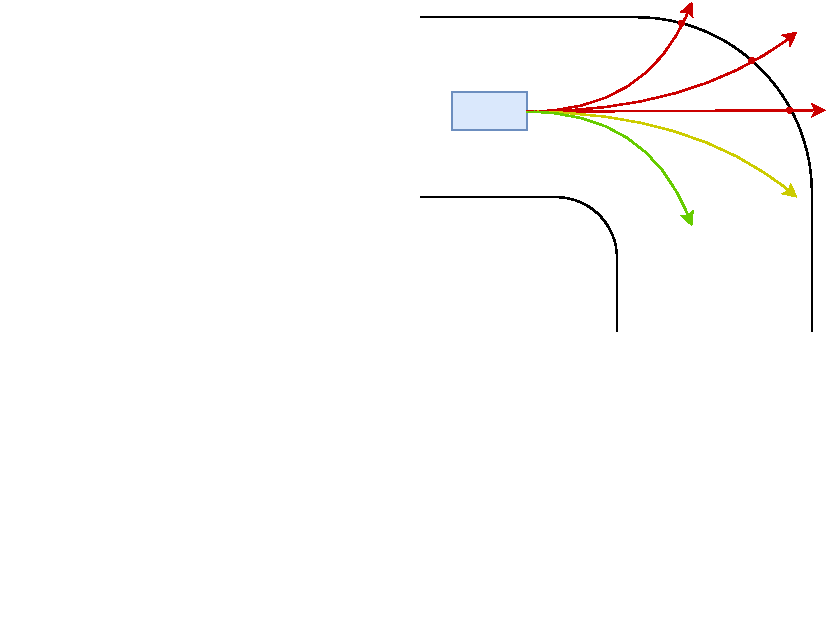
\includegraphics[trim=200 170 0 0, clip, width=0.75\textwidth]{../img/dwa_tentacles}
	\caption{Application of different actions can be visualized as a set of ``tentacles'' around the vehicle. Each ``tentacle'' is a prediction of the positions of the vehicle during the prediction horizon period. Each of the predicted trajectories is scored and the action which produces the best trajectory is selected.}
	\label{fig:dwa}
\end{figure}

At each time when we want to select the next control input for our vehicle, the DWA algorithm \cite{DWA} samples the control space of the robot and simulates the trajectories which the robot would travel if the action was applied for a short time period $T=k\cdot \Delta t,k\in\mathbb{N}$. The resulting trajectories, which do not result in a collision, are scored and the action of the best trajectory is used. The outline of the algorithm adapted for our problem can be seen in Algorithm~\ref{alg:dwa} and it is visualized in Figure~\ref{fig:dwa}.

\begin{algorithm}
	\SetAlgoLined
	\DontPrintSemicolon
	
	\SetKwFunction{DWA}{DWA}
	\SetKwFunction{Unfold}{Unfold}
	\SetKwFunction{EmergencyStop}{EmergencyStop}
	
	\KwIn{Collision detection function $c$, time step $\Delta t$, finite set of actions $U_f$, horizon $k\in\mathbb{N}$}
	\KwOut{An action $u\in U_f$}
	\Parameter{Initial state $x_0$, reference trajectory $\hat{x}_{ref}$}
	
	\SetKwProg{algorithm}{Algorithm}{:}{}
	
	\BlankLine
	
	\algorithm{\DWA{$x_0$, $\hat{x}_{ref}$}}{
		$T\gets \emptyset$\;
		\ForEach{$u\in U_f$}{
			$\hat{x}'\gets $ \Unfold{$x_0$, $u$, $k$, $\Delta t$}\;
			\If{$\forall x\in \hat{x}': c(x)=F$}{
				$T\gets T\cup\left\{\hat{x}'\right\}$\;
			}
		}
	
		\If{$T=\emptyset$}{
			\KwRet{\EmergencyStop{}}\;
		}
	
		\KwRet{$\argmin_{\hat{x}\in T} \hat{e}_{\Delta t}(\hat{x})$}\;
	}
		
	\caption{Dynamic Window Approach}
	\label{alg:dwa}
\end{algorithm}

The function \texttt{Unfold} simulates the motion of the vehicle from the state $x_0$ using the control command $u$ in the next $k$ steps and returns the state trajectory which is obtained.

The function \texttt{EmergencyStop} is used when there is no valid trajectory and it selects a control input from the set of possible actions which will slow down the vehicle as much as possible before hitting the obstacle.

The time complexity of the algorithm is $O(k\cdot n)$ and it requires $O(k\cdot n)$ of memory, for $n=|U_f|$. Since both values are small constants, the algorithm itself can be very fast and the delay $t_d$ will be low.

The algorithm prefers trajectories which will bring the vehicle closer to the reference trajectory while avoiding collisions with any obstacles along the trajectory which might not have been known during the planning phase.

